\chapter{云计算基础}

\section{产生背景}

\subsection{云计算之前的技术}

\begin{definition}[并行计算]
    同时使用多种计算资源解决计算问题的过程,主要目的是快速解决大型且复杂的计算问题。

\end{definition}

并行计算把计算任务分派给系统内的多个运算单元。\term{HPC} server, 使用一个强大的机器或者infiniband 万兆网络连接,分派给系统中的多个运算单元;共享memory(可以直接访问所有内存)

\begin{definition}[InfiniBand]
    InfiniBand 是指具有非常高的RAS(可靠性、可用性、维护性)的基础设施/高性能计算机的服务器/集群用高速I/O总线架构及互联。作为系统间互联结构,除了RAS功能以外,与其他机构相比,具有低延迟这一点也是其特征。
\end{definition}

\begin{definition}[分布式计算]
    把一个需要巨大的计算能力才能解决的问题分成多个小部分,把这些小部分分配给多个计算进行处理,最后综合这些计算结果得到最终结果。
\end{definition}

分布式计算在cluster上运行,使用百兆网络等; 将计算任务分派给多个机器,再merge;分布式memory,需要进行消息传送

快速的分布式:MapReduce, Hadoop, spark

\begin{definition}[网格计算]
    利用互联网把地理上广泛分布的各种资源连成一个逻辑的整体,就像一台超级计算机一样。
\end{definition}

\begin{example}[教育网格]
    学校信息中心计算队列:将空闲的服务器通过教育网共享

    特点: 网格服务器一般不断电:软件configuration,路径,环境变量重启之后需要重新设置麻烦;逻辑上分布在不同机器上的程序是连续的,初期教育网格没有进行虚拟化
    缺点: 需要提供自己的计算资源,限制成员
\end{example}

\begin{definition}[云计算]
    一种基于互联网的计算方式. 通过网络,提供按需、且易扩展的弹性计算以及应用服务。
\end{definition}

云计算有anyone, anytime, anywhere的特点; 共享软硬件, 有些平台提供shared licenses的软件; 按需易拓展 autoscaling; 

\begin{figure}[htbp]
    \centering
    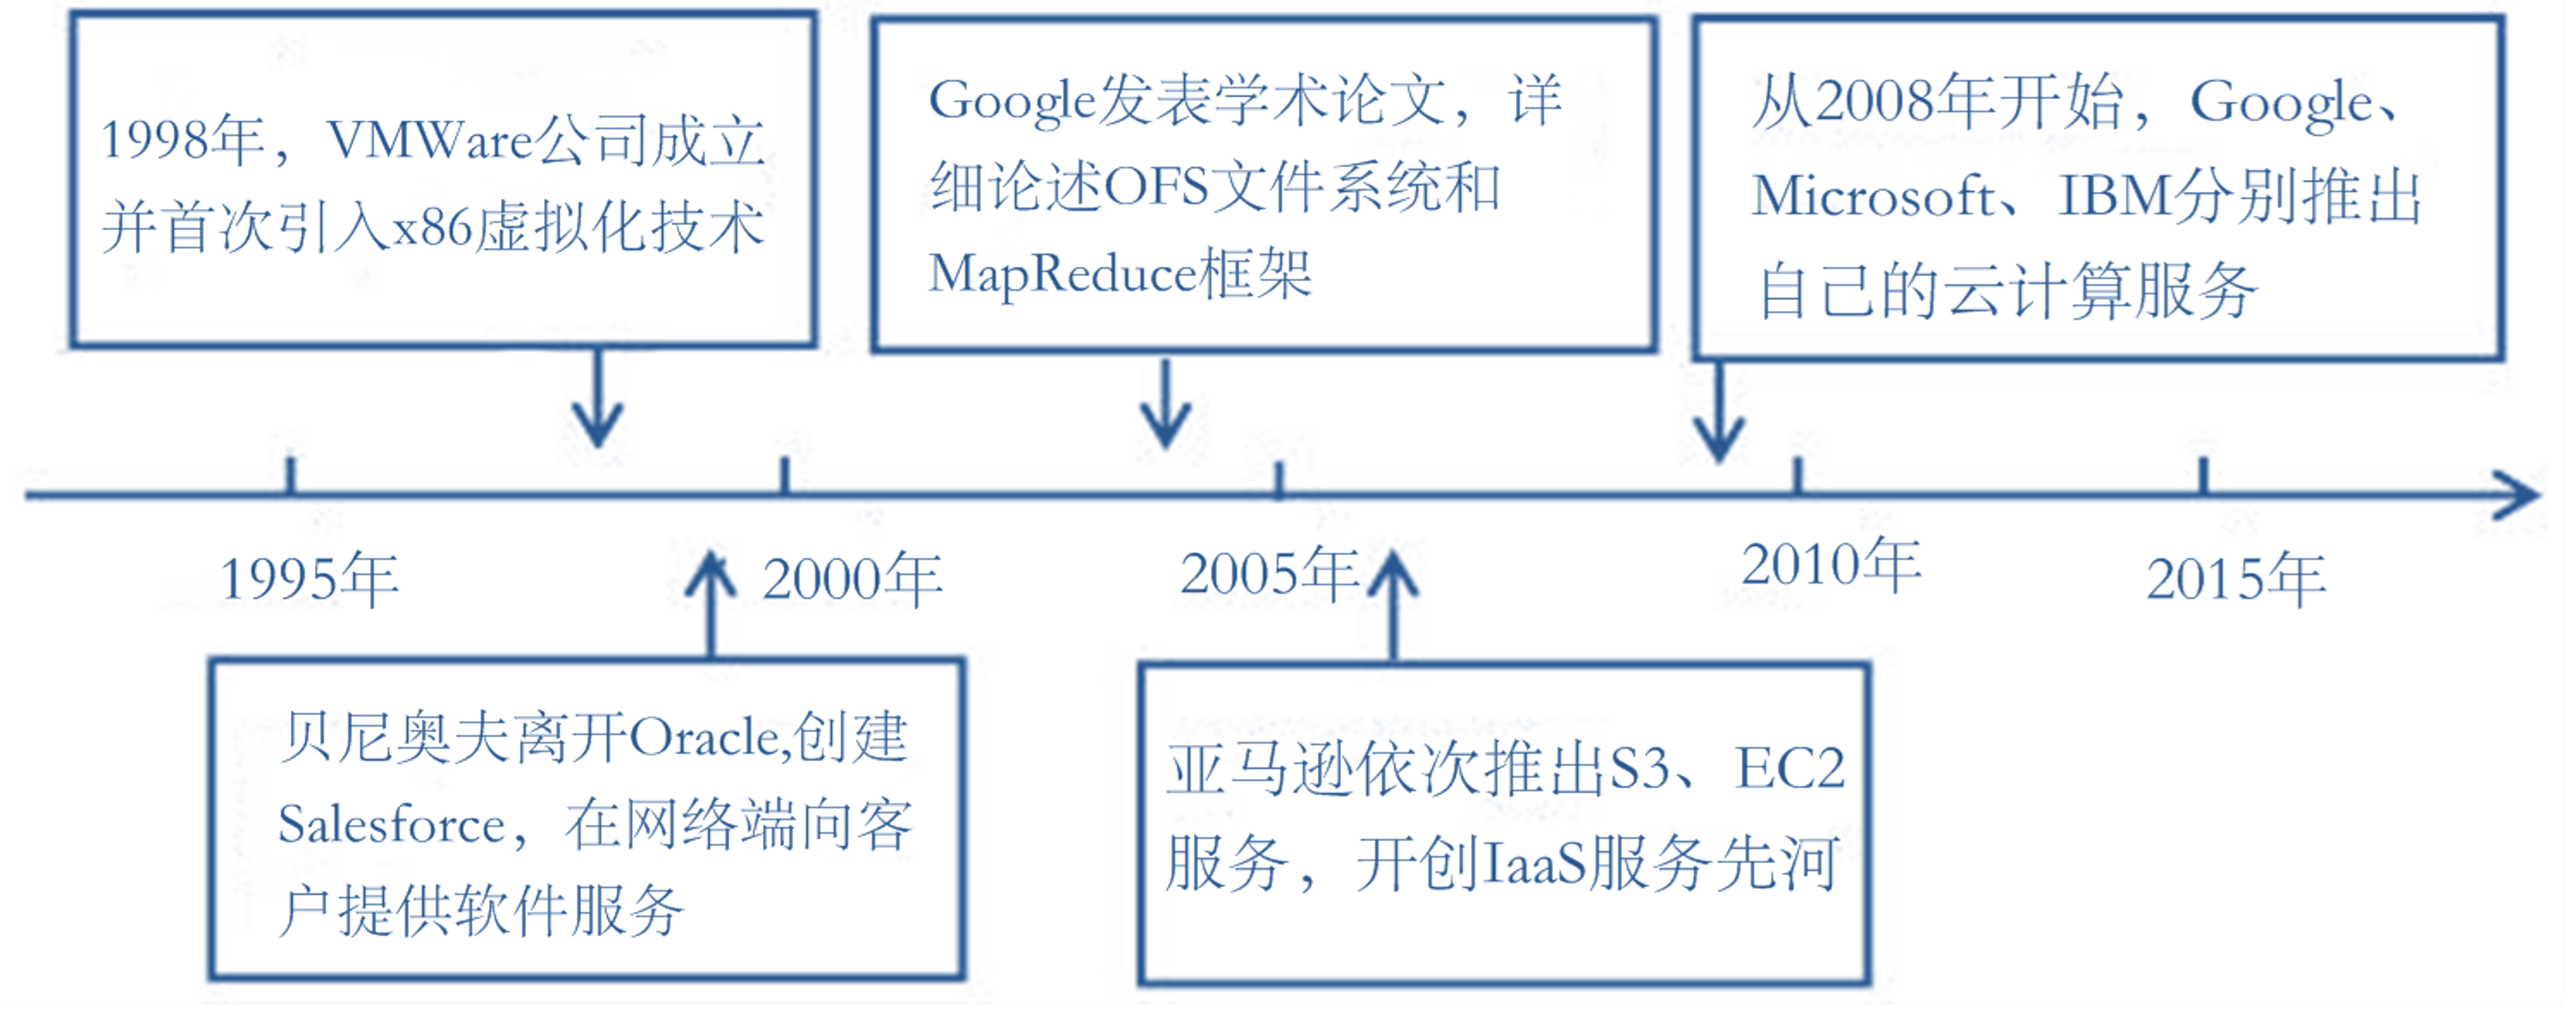
\includegraphics{cloud-development-of-cloud-computing.png}
\end{figure}

\subsection{其他技术的发展}

\begin{itemize}
    \item 5G
    \item 移动互联网
    \item 物联网
\end{itemize}

\subsection{国外云计算厂商}

亚马逊的云计算称为Amazon Web Services(AWS).率先在全球提供了弹性计算云EC2(Elastic Computing Cloud)和简单存储服务S3(Simple Storage Service),为企业提供计算和存储服务。收费的服务项目包括存储空间、带宽、CPU资源以及月租费。AWS服务的种类非常齐全. 
机器,计费使用时长(以小时, 分钟再到按照秒计算)等数据模型变化,技术不断进步.

\begin{definition}[Amazon Elastic Compute Cloud]
    Amazon Elastic Compute Cloud(Amazon EC2 云服务器)是一种 Web 云服务,能在云中提供安全且可调整大小的计算能力。该服务旨在让开发人员能够更轻松地进行 Web 规模的云计算。Amazon EC2 云服务器的 Web 云服务接口非常简单,您可以最小的阻力轻松获取容量,随之配置容量。使用该服务,您将能完全控制您的计算资源,并能在亚马逊成熟且行之有效的计算环境中运行。

    Amazon EC2 云服务器提供最广泛、最深入的计算平台,可选择处理器、存储、联网、操作系统和购买模式。我们提供最快的云处理器,是唯一的 400 Gbps 以太网网络云。我们拥有最强大的针对机器学习培训和图形工作负载的 GPU 云服务器实例,以及云中每次推理成本最低的云服务器实例。与任何其它云相比,AWS 均运行更多的 SAP、HPC、机器学习和 Windows 工作负载。单击此处了解 Amazon EC2 云服务器的最新功能。
\end{definition}

\begin{definition}[Serverless]
    开发者再也不用过多考虑服务器的问题,计算资源作为服务而不是服务器的概念出现。Serverless是一种构建和管理基于微服务架构的完整流程.

    (AWS 上的无服务器)无服务器是一种用于描述服务、实践和策略的方式,使您能够构建更敏捷的应用程序,从而能够更快地创新和响应变化。凭借无服务器计算,容量预置和补丁等基础设施管理任务由 AWS 处理,以便您能够专注于编写为客户服务的代码。AWS Lambda 等无服务器服务具有自动扩展、内置高可用性以及按价值付费的计费模型。Lambda 是一种事件驱动的计算服务,使您能够运行代码来响应来自 200 多个本地集成的 AWS 和 SaaS 源的事件 — 所有这些都无需管理任何服务器。
\end{definition}

\begin{definition}
    AWS Lambda 是一种无服务器的计算服务,让您无需预置或管理服务器、创建可感知工作负载的集群扩展逻辑、维护事件集成或管理运行时,即可运行代码。借助 Lambda,您几乎可以为任何类型的应用程序或后端服务运行代码,而且完全无需管理。只需将您的代码以 ZIP 文件或容器映像的形式上传,Lambda 便会自动、精确地分配计算执行能力,并根据传入的请求或事件运行您的代码,以适应任何规模的流量。您可以将您的代码设置为自动从 200 多个 AWS 服务和 SaaS 应用程序触发,或者直接从任何 Web 或移动应用程序调用。您可以使用自己喜欢的语言(Node.js、Python、Go、Java 等)编写 Lambda 函数,并使用无服务器和容器工具(例如 AWS SAM 或 Docker CLI)来构建、测试和部署您的函数。
\end{definition}

\begin{definition}[(腾讯云)云函数]
    腾讯云云函数是腾讯云提供的 Serverless 执行环境。您只需编写简单的、目的单一的云函数即可将它与您的腾讯云基础设施及其他云服务产生的事件关联。

使用云函数时,您只需使用平台支持的语言(Python、Node.js、PHP、Golang、Java 及 Custom Runtime)编写代码。腾讯云将完全管理底层计算资源,包括服务器 CPU、内存、网络和其他配置/资源维护、代码部署、弹性伸缩、负载均衡、安全升级、资源运行情况监控等。但这也意味着您无法登录或管理服务器、无法自定义系统和环境。

云函数自动地在同一地域内的多个可用区部署,同时提供极高的容错性。云函数在执行时将根据请求负载扩缩容,从每天几个请求到每秒数千个请求,都由云函数底层自行伸缩。您无需人工配置和介入,只需为运行中的云函数付费,即可满足不同情景下服务的可用性和稳定性。若云函数未运行,则不产生任何费用。

您可以自定义运行云函数的时机,例如,在 COS Bucket 上传时、删除文件时运行云函数、使用 Ckafka 中的消息时运行云函数、应用程序通过 SDK 调用时运行云函数,或指定云函数定期执行。您可以使用云函数作为 COS 服务的数据处理触发程序轻松实现 IFTTT 逻辑,您也可以通过构建灵活的定时自动化任务,用于覆盖手工完成的操作,轻松构建灵活可控的软件架构。

\begin{itemize}
    \item 简单易用: 用户只需编写最重要的“核心代码”,不再需要关心周边组件,极大地降低了服务架构搭建的复杂性。无需任何手动配置,云函数即可根据请求量自动横向扩缩。不管您的应用每天的请求数处于波峰还是波谷,云函数均可自动安排合理的计算资源满足业务需求。
    \item 高效: 云函数不要求特定框架,开发者可专注于核心代码的开发。单个模块的开发无需了解代码细节。您可以使用云函数编写一些目的单一、逻辑独立的业务模块。每个函数都是单独运行、单独部署、单独伸缩的,用户上传代码后即可自动部署,提升了独立开发和迭代的速度。
    \item 稳定可靠: 如果某个可用区因灾害或电力故障等导致瘫痪,云函数会自动地选择其他可用区的基础设施来运行,免除单可用区运行的故障风险。由事件触发的工作负载可以使用云函数来实现,利用不同云服务满足不同的业务场景和业务需求,使得您的服务架构更加健壮。
    \item 简化管理: 用户不再需要对 OS 入侵、登录风险、文件系统安全、网络安全和端口监听做复杂的配置和管理,一切交由平台处理,平台通过定制化的容器保证每个用户的隔离性。用户无需复杂的配置文件即可一键部署和测试云函数。
    \item 降低开销: 云函数在未执行时不产生任何费用,所以对一些无需常驻的业务进程来说,开销将大幅降低。云函数执行时按请求数和计算资源的运行时间收费,价格优势明显,对初创期的开发者十分友好。
\end{itemize}
\end{definition}

谷歌是最大的云计算技术的使用者. 谷歌已经允许第三方在谷歌的云计算中通过\term{Google App Engine}运行大型并行应用程序. 发表学术论文的形式公开其云计算三大法宝:\term{Google File System} (GFS)、\term{MapReduce}和\term{BigTable}. 基于TensorFlow


微软紧跟云计算步伐,推出了Microsoft Azure. 微软将为Windows Azure用户推出许多新的功能,不但能更简单地将现有的应用程序转移到云中,而且可以加强云托管应用程序的可用服务,充分体现 出微软的“云”+“端”战略。在中国,微软2014年3月27日宣布由世纪互联负责运营的Microsoft Azure公 有云服务正式商用,这是国内首个正式商用的国际公有云服务平台。

\begin{figure}[htbp]
    \centering
    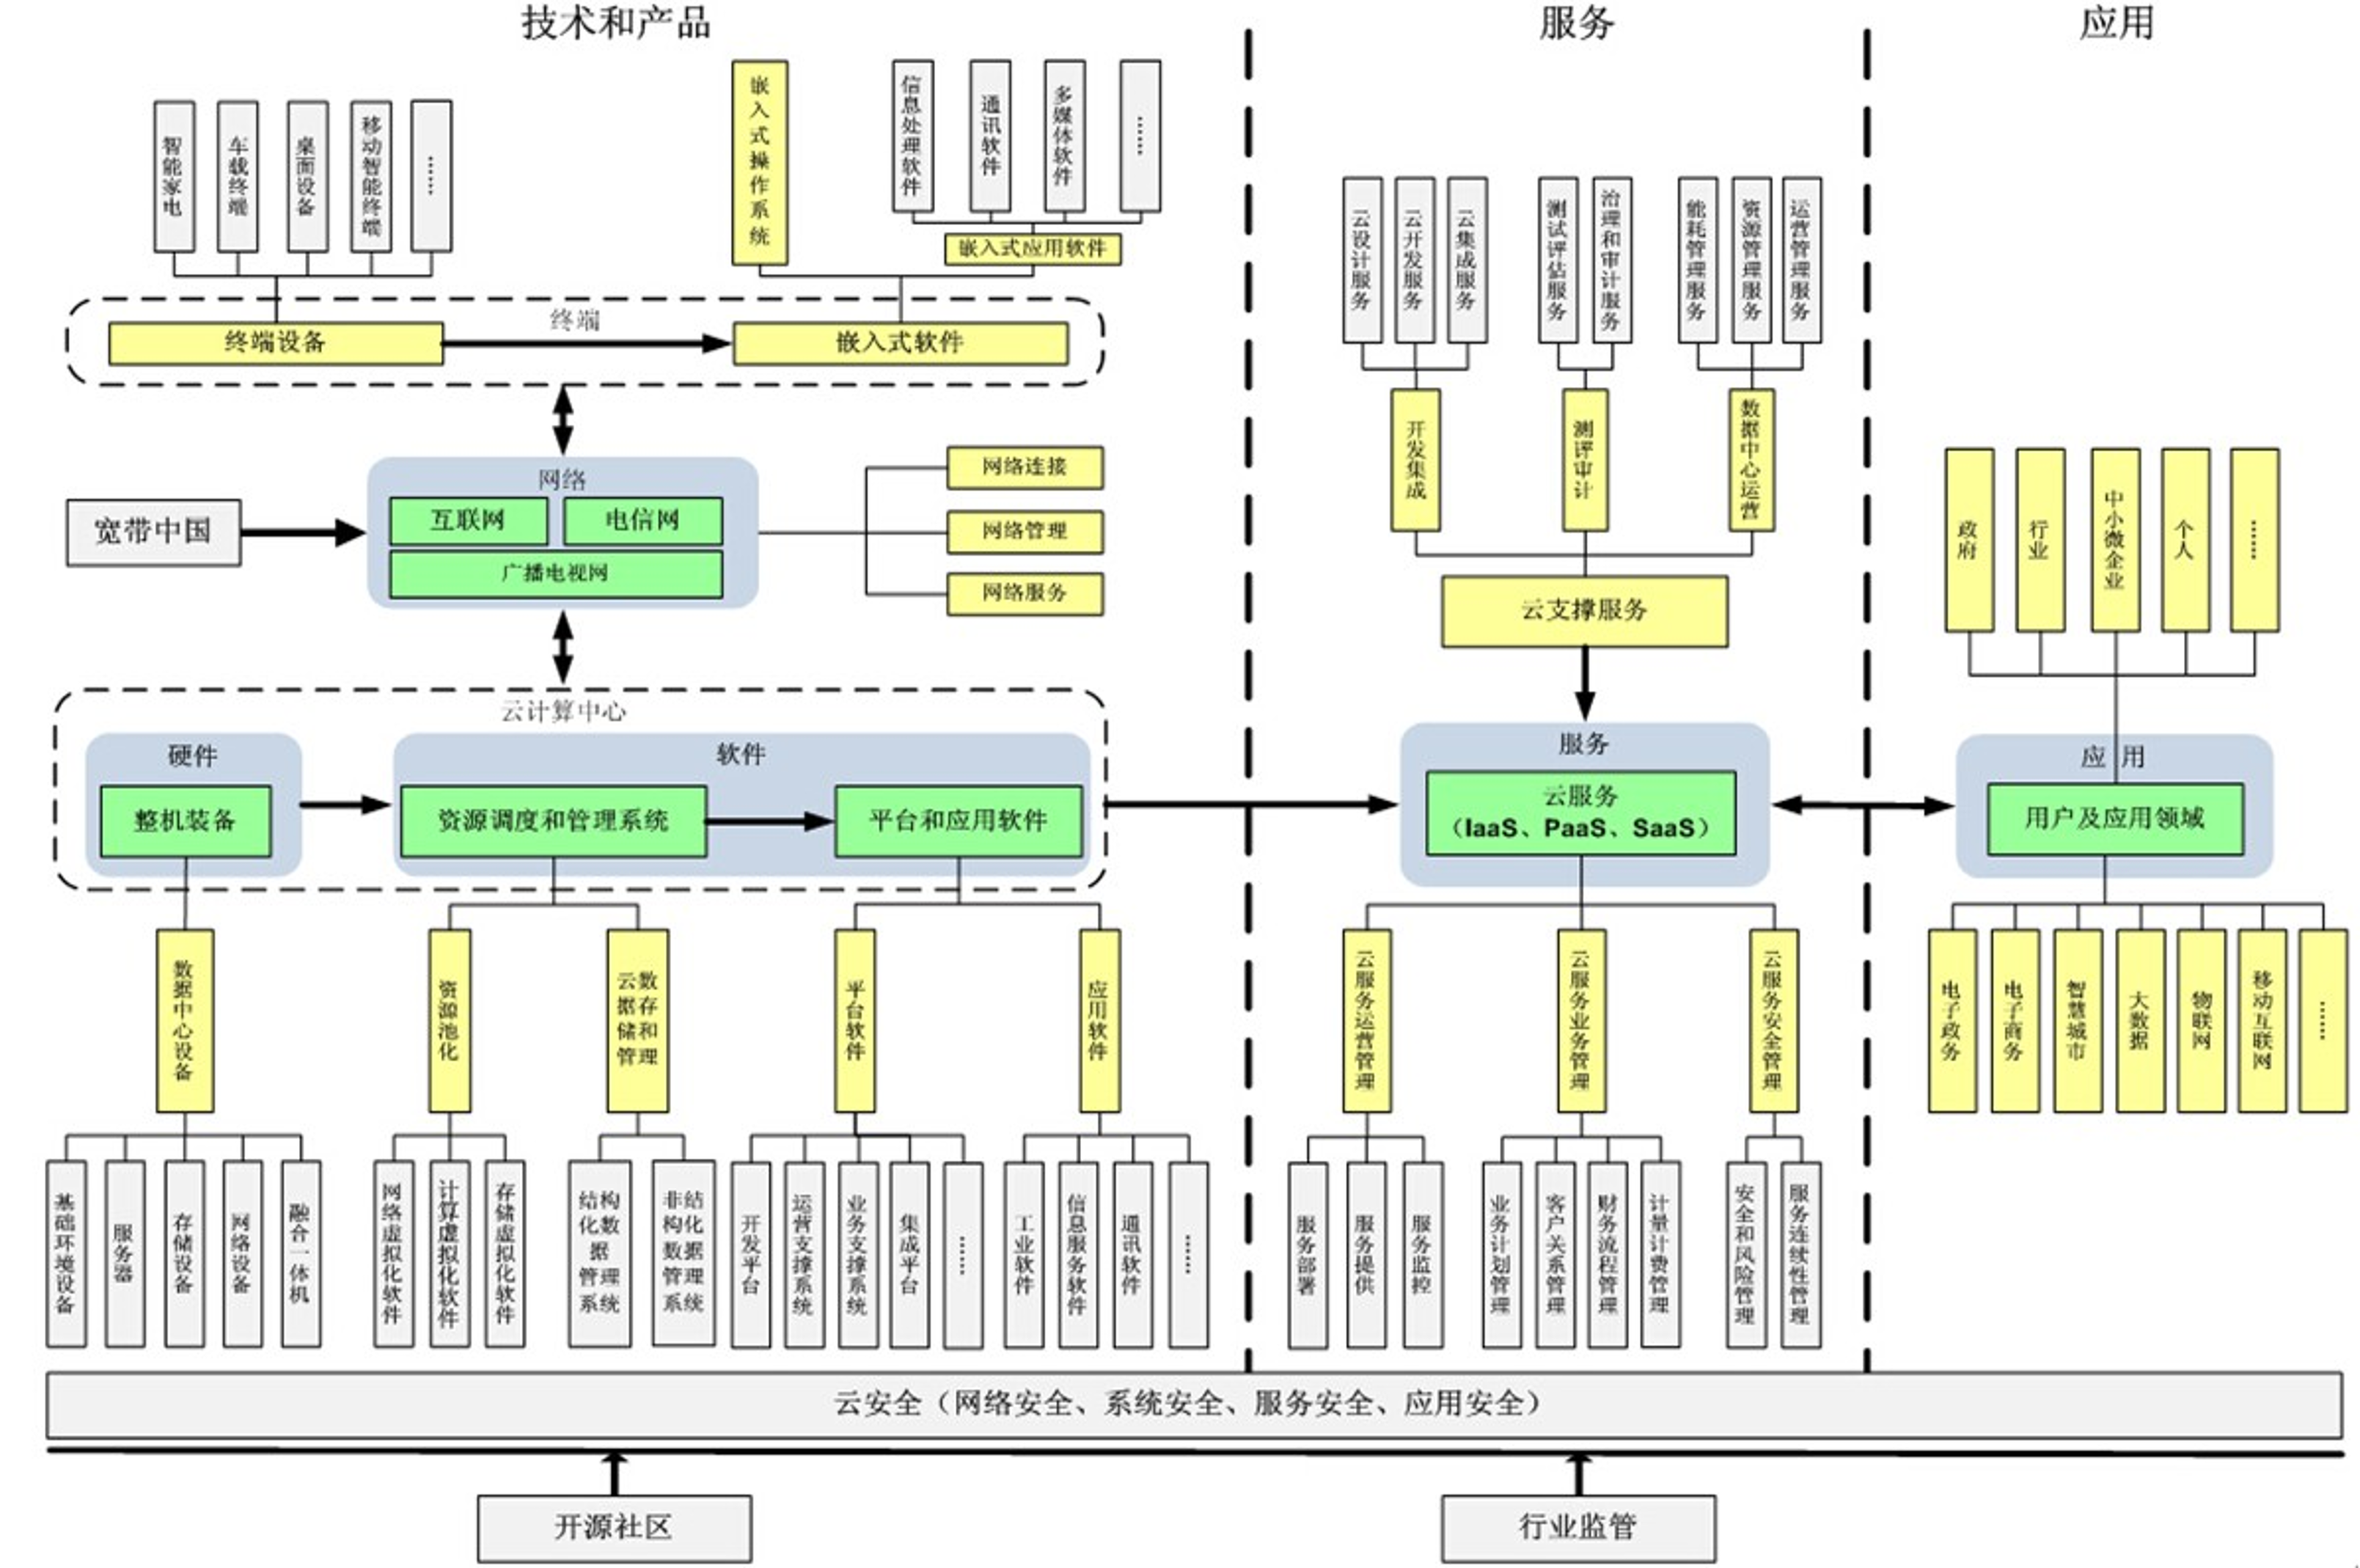
\includegraphics{cloud-cloud-computing-biosphere.png}
\end{figure}

\subsection{其他原因}

个人使用计算机的不灵活性:

\begin{itemize}
    
    
    \item 刚高价购买的最新版的应用程序,过了不久就需要进行更新
    \item 你刚刚购买完电脑,就出现了新的型号
    \item 电脑因为太多的不灵活的软件,负载过重而宕机,导致保存的数据全部丢失
    \item 一时冲动购买了一套软件,结果用了不到一个月就失去了兴趣
\end{itemize}

企业使用计算机的不灵活性:

\begin{itemize}
    
    
    \item IT部门的工作人员经常忙于穿梭于各个办公楼之间解决员工电脑的各种系统错误,各种应用软件的错误
    \item 企业为了测试新开发的应用软件,需要购买一大批电脑,而当测试完毕之后,大部分设备处于闲置
    \item 为了应付市场的快速变化,急需一批计算资源,但是审批资金、购买设备、安装平台可能需要花费2周左右的时间,会耽误市场机会
    \item 高价购买了某家公司的软件之后,使用一段时间之后,发现不能完全满足需求,但是又无法退货
\end{itemize}

云计算提出前的互联网遇到的难题:
\begin{itemize}
    \item \textbf{互联网上的数据量高速增长}(\term{Big Data}),导致了互联网数据处理能力的不足;
    \item 互联网上存在着大量处于闲置状态的计算设备和存储资源;
    \item 服务器更新换代速度加快,企业升级费用昂贵。
\end{itemize}

\section{云计算与大数据}

\begin{definition}[Big Data]
    海量数据或巨量数据,其规模巨大到无法通过目前主流的计算机系统在合理时间内获取、存储、管理.
\end{definition}

\subsection{大数据的特征}

\begin{itemize}
    \item 价值密度低(Value):(需要挖掘数据,数据清洗:重复、无用、噪声数据、缺失值处理)在成本可接受的条件下,通过快速采集、发现和分析,从大量、多种类别的数据中提取价值的体系架构。

    \item 快速(Velocity):数据增长速度快,而且越新的数据价值越大,这就要求对数据的处理速度也要快,以便能够从数据中及时地提取知识,发现价值。(产生速度快,数据处理需要高效率) 例如\term{Streaming Processing}:如果处理速率不够快,会\term{丢包}; zoom 多方会议,带宽有限,如何进行数据传输调度?$\rightarrow$用户体验提升

    \item 数据量大(Volume):存储的数据量巨大,PB级别是常态,因而对其分析的计算量也大。

    \item  多样(Variety):数据的来源及格式多样,数据格式除了传统的结构化数据外,还包括\term{半结构化数据}或\term{非结构化数据}(如搜索喜马拉雅:只能搜索\term{metadata}(文件名/小说名/属性等),无法根据内容中的某个细节搜索 $\rightarrow$ \term{非结构化数据索引})。而随着人类活动的进一步拓宽,数据的来源更加多样。

   \item 复杂度(Complexity):对数据的处理和分析的难度大。

   $$G=f(x), f:\text{云计算}, x:\text{大数据}$$
\end{itemize}



\section{云计算基本思想 (通用性)}

\begin{itemize}
    \item 基本能力(所有的计算能力、存储能力、和各种各样功能的应用)都可通过网络获得
    \item 云应对用户硬件友好, 不需要不停地更换昂贵的高性能电脑
    \item 不需要用户安装复杂软件
    \item  数据保证安全(备份)
\end{itemize}

\term{三备份},仍旧可能会丢失